
\documentclass[10pt,cn]{elegantbook}
\usepackage[utf8]{inputenc}
\usepackage[T1]{fontenc}
\usepackage{tgtermes}
\usepackage{amsmath}
\usepackage{amsfonts}
\usepackage{amssymb}
\usepackage{stmaryrd}
\usepackage{hyperref}
\hypersetup{colorlinks=true, linkcolor=blue, filecolor=magenta, urlcolor=cyan,}
\urlstyle{same}
\usepackage{graphicx}
\usepackage[export]{adjustbox}
\usepackage{mdframed}
\usepackage{booktabs,array,multirow}
\usepackage{esint}
\usepackage{xeCJK}
%\usepackage{adjustbox}
\usepackage[export]{adjustbox}
%\graphicspath{ {./images/} }

\usepackage{ulem}
\usepackage{hyperref}%目录跳转

\usepackage{fontspec} % 用于处理字体
%\setmainfont{TeX Gyre Termes} % 设置主要字体


%\usepackage{fancyhdr}   % 导入 fancyhdr 包,用于定制页眉和页脚
%\usepackage{datetime}   % 导入 datetime 包,用于格式化日期


\usepackage{graphicx}   % 导入 graphicx 包,以便插入图片


\usepackage{comment}

%\fancyhead[L]{20240722} % 左侧页眉
%\fancyhead[R]{\mydate\today} % 右侧页眉,显示当前日期,格式为“日 月 年”

\title{HappaChemistryNotes}
\subtitle{化学笔记}
\author{OyamaHappa}
\date{\today}
\version{20240725090259}
\extrainfo{孔明是我的理想,商鞅是我的下场}
\logo{logo.jpg}
\cover{cover.jpg}



% 本文档命令
\usepackage{array}
\usepackage{mathdots}
\newcommand{\ccr}[1]{\makecell{{\color{#1}\rule{1cm}{1cm}}}}
% 修改目录深度
\setcounter{tocdepth}{3}

\everymath{\displaystyle}%用行间公式(displaystyle)的格式排版所有的行内公式


%\usepackage{verbatim}%在codeshow中已引用
\usepackage{tikz,tkz-euclide}
\usepackage{amsmath}
\usepackage{pgfplots}
%\usepackage{codeshow}%codeshow:为了在codeshow环境中,引用代码,并生成图形。

\usepackage{graphicx}
%\usepackage{subfigure}

\usepackage{breqn}%breqn 宏包主要提供了 dmath 和 dmath* 等几个环境,产生可以自动折行的显示公式。
\usepackage{longtable}%长表格,多页可以自动处理。

%【参与编译的文件列表。】
%\includeonly{preface,chapter01,chapter02,chapter03,chapter04,chapter05}%,%【参与编译的文件列表。】




\usepackage{amsmath}
\usepackage{amsfonts}
\usepackage{amssymb}
\usepackage{stmaryrd}
\usepackage{hyperref}
\hypersetup{colorlinks=true, linkcolor=blue, filecolor=magenta, urlcolor=cyan,}
\urlstyle{same}
\usepackage{graphicx}
\usepackage[export]{adjustbox}
\usepackage{mdframed}
\usepackage{booktabs,array,multirow}
\usepackage{esint}
\usepackage{xeCJK}
\usepackage{adjustbox}
\newcommand{\HRule}{\begin{center}\rule{0.5\linewidth}{0.2mm}\end{center}}
%\graphicspath{ {./images/} }
\usepackage{amsmath}
\usepackage{pifont}


\begin{document}
	
	\begin{titlepage}
		\begin{center}
			\vspace*{3cm}
			
			{\Large \textbf{HappaNotesBooks} }
			
			{\Large(试 用)}
			
			\vspace{1cm}
			
			{\Huge 化 \qquad 学}
			
			\vspace{0.5cm}
			
			
			
			
			
			
			\vspace{1cm}
			
		OyamaHappa
			
			\vfill
			
			
			孔明是我的理想,商鞅是我的下场
			
			
			
		\end{center}
	\end{titlepage}
	
%	\maketitle
	
	\tableofcontents
	%\listofchanges
	
	\mainmatter

	\part{化学反应原理}
    \chapter{中和滴定实验}
	\section{滴定实验}
	
	我们在研究物质时, 常常需要对物质进行定性分析和定量分析。确定物质的成分, 包括元素、 无机物所含的离子和有机物所含的官能团等, 在化学上叫做定性分析。测定物质中元素、离子、官能团等各成分的含量, 在化学上叫做定量分析。
	
	%【思考】现有一瓶未知浓度的 \(\mathrm{{NaOH}}\) 溶液,如何准确测出其浓度?
	
	\subsection{酸碱中和滴定}
	
	利用中和反应原理, 用已知物质的量浓度的酸 (或碱) 来测定未知物质的量浓度的碱 (或酸) 的方法
	
	1、中和反应:
	
	2、中和滴定原理:
	
	\[
	\mathrm{{HA}} + \mathrm{{BOH}} = \mathrm{{BA}} + {\mathrm{H}}_{2}\mathrm{O}
	\]
	
%	\(1\mathrm{\;{mol}}\;1\mathrm{\;{mol}}\)
	
	即可得 \({\mathrm{c}}_{\left( \mathrm{{HA}}\right) }{\mathrm{V}}_{\left( \mathrm{{HA}}\right) } = {\mathrm{c}}_{\left( \mathrm{{BOH}}\right) }{\mathrm{V}}_{\left( \mathrm{{BOH}}\right) }\)
	
	现在我们用 \({0.1000}\mathrm{\;{mol}}/\mathrm{L}\) 的 \(\mathrm{{HCl}}\) 溶液测定未知浓度的 \(\mathrm{{NaOH}}\) 溶液,到底应测得哪些数据才能求出 \({\mathrm{c}}_{\left( \mathrm{{NaOH}}\right) }\) ?
	
	\begin{center}
		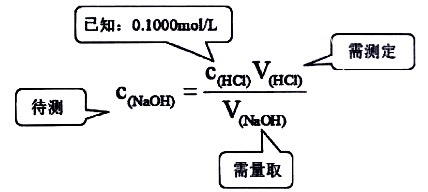
\includegraphics[max width=0.5\textwidth]{image/c1.jpg}
	\end{center}
	
	\subsection{滴定实验仪器以及操作要点}
	
	\subsubsection{滴定方法的关键}
	
	(1)准确测定两种反应物溶液的体积
	
	(2)确保标准液、待测液浓度的准确
	
	(3)\uline{滴定终点的准确判定}(包括指示剂的合理选用)
	\subsubsection{实验仪器及试剂}
	
	\begin{center}
		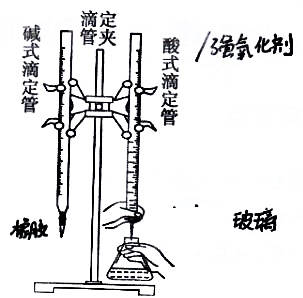
\includegraphics[max width=0.2\textwidth]{image/c2-1.jpg}
	\end{center}
	
	(1)仪器:酸式滴定管、碱式滴定管、滴定管夹、烧杯、锥形瓶、铁架台。
	
	\begin{center}
		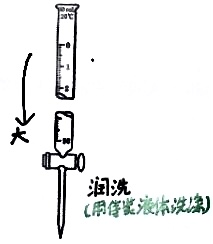
\includegraphics[max width=0.2\textwidth]{image/c2-2.jpg}
	\end{center}
	\[\mbox{酸式滴定管}\]
		\[\mbox{润洗--用待装液体洗涤}\]
	\begin{center}
		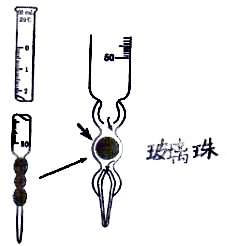
\includegraphics[max width=0.2\textwidth]{image/c2-3.jpg}
	\end{center}
		\[\mbox{碱式滴定管}\]
	 
	
	\subsubsection{滴定管的构造特点}
	
		\ding{172}标识: 标有温度、刻度、规格(25.00 mL 或 \({50.00}\mathrm{\;{mL}}\) )%圈1
	
	\ding{173}刻度:零刻度在\_\_\_,满刻度在\_\_\_;最小刻度为 0.1 ml,精确度为 0.01 ml。%圈2
	
	\ding{174}酸式滴定管: 下端是玻璃塞, 能盛装 \_溶液;
	
	碱式滴定管: 下端是橡皮管+玻璃小球, 能盛装\_
	
	%【思考 1】现在要量取 \({25.00}\mathrm{\;{mL}}\mathrm{{NaOH}}\) 溶液,应该用什么量取? 能不能用量筒? 为什么?
	
%	【思考 2】如图是某些仪器的刻度部分示意图, 图中各仪器虚线为所示读数。其中为量筒的是 \_\_\_(填编号,下同),读数为 \(2\text{、}n\mathrm{\;L}\) ;为滴定管的是\_\_\_,读数为 \(2\text{、}\mathrm{{SmL}}\)
	
%	\begin{center}
	%	\includegraphics[max width=0.3\textwidth]{images/0190d453-f338-754b-8cea-9ab8ce034fb0_0_605307.jpg}
	%\end{center}
	
%	① \ding{173}
	\subsubsection{凡士林的涂抹方式}
	
	\begin{center}
		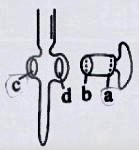
\includegraphics[max width=0.2\textwidth]{image/c3-1.jpg}
	\end{center}
	
		\[\mbox{涂a和c}\]
	
	
	润洗仪器: 在加入酸、碱之前, 洁净的酸式滴定管和碱式滴定管要分别用所要盛装的酸、碱润洗 \(2 \sim 3\) 次。
	
	\ding{173}方法是: 从滴定管上口加入 \(3 \sim 5\mathrm{\;{mL}}\) 所要盛装的酸溶液或碱溶液。倾斜着转动滴定管,使液体润湿全部滴定管内壁。然后, 一手控制活塞 (轻轻转动酸式滴定管的活塞; 或者轻轻挤压碱式滴定管中的玻璃球),将液体从滴定管下部放入预置的烧杯中。
	
	\ding{174}加入反应液: 分别将酸溶液、碱溶液加到酸式滴定管、碱式滴定管中,\uwave{ 使液面位于滴定管刻度“0”以上 \(2 \sim 3\mathrm{\;{mL}}\) 处},并将滴定管垂直固定在滴定管夹上。
	
	
	\ding{175}调节起始读数: 在滴定管下放一个烧杯, 调节活塞, 使滴定管尖嘴部分充满反应液, 并使液面处于“0”刻度(或“0”刻度以下),准确读取读数并记录$¥V_{\mbox{始}}$
	
	【思考 7】如果滴定管内出现气泡怎么排出气泡? 
	
	排气泡: 酸式滴定管 \(\rightarrow\)尖嘴部分朝上,碱式滴定管\(\rightarrow\)
	
	\begin{center}
		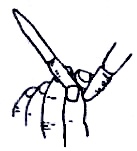
\includegraphics[max width=0.2\textwidth]{image/c4-1.jpg}
	\end{center}
		\[\mbox{除去碱式滴定管乳胶管中气泡的方法}\]
	
	
	\ding{176} 放液
	
	a 从碱式滴定管中放出 \({25.00}\mathrm{{ml}}\) 氢氧化钠溶液于锥形瓶中;
	
	
	
	\(\mathrm{b}\) 滴入几滴\uwave{酚酞试液}(指示剂),将锥形瓶置于酸式滴定管下方,并在瓶底衬一张白纸。
	
		\ding{177}滴定: 左手控制酸式滴定管活塞, 右手摇动锥形瓶, 边滴入盐酸 (当接近终点时, \uwave{改为滴加半滴酸}) , 边不断顺时针方向摇动, 眼睛要始终注视
	
	\begin{center}
		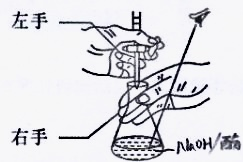
\includegraphics[max width=0.3\textwidth]{image/c4-2.jpg}
	\end{center}
	
	\ding{178}记读数: $\star$ \uwave{当滴入最后半滴HCl,溶液由红色突变为无色,且半分钟内不褪色. 停止滴定,准确记下盐酸读}数 \({\mathrm{V}}_{\text{终}}\) ,并准确求得滴定用去的盐酸体积 \(\mathrm{V} = {\mathrm{V}}_{\text{始 }} - {\mathrm{V}}_{\text{终 }}\) (平行实验 2 -3 次) 
	
	滴入最后半滴标准溶液具体操作?
	
	\ding{179}计算
	
	【经典 2】【2020 年 7 月选考】滴定前, 有关滴定管的正确操作为 (选出正确操作并按序排列,选项可重复使用): 检漏 \(\rightarrow\) 蒸馏水洗涤 \(\rightarrow\) 用滴定液润洗 2 至 3 次 \(\rightarrow\) 装入滴定液至零刻度以上 \(\rightarrow\) 排除气泡 \(\rightarrow\) 调整滴定液液面至零刻度或零刻度以下\( \rightarrow \)记录起始读数 \(\rightarrow\) 开始滴定。
	
	
\subsection{指示剂的选择}

\subsubsection{酸碱指示剂}

(1)酸碱指示剂的变色范围(pH 值) 

\begin{center}
	\adjustbox{max width=\textwidth}{
		\begin{tabular}{|c|c|c|c|}
			\hline
			\multirow{2}{*}{甲基橙} & \(< {3.1}\) & \({3.1} \sim {4.4}\) & \(> {4.4}\) \\
			\hline
			& 红 & 橙 & 黄 \\
			\hline
			\multirow{2}{*}{酚酞} & \(< {8.2}\) & \({8.2} \sim {10}\) & \(> {10}\) \\
			\hline
			& 无色 & 浅红 & 红 \\
			\hline
			\multirow{2}{*}{石蕊} & \(< 5\) & \(5 \sim 8\) & \(> 8\) \\
			\hline
			& 红 & 紫 & 蓝 \\
			\hline
		\end{tabular}
	}
\end{center}
\paragraph{滴定终点}

\[\mbox{显酸}\Rightarrow\mbox{甲基橙}\]
\[\mbox{显碱}\Rightarrow\mbox{酚酞}\]
\paragraph{变化曲线}

若以酸碱中和滴定过程中滴加酸 (或碱) 的量为横轴,以溶液的 \(\mathrm{{pH}}\) 为纵轴,即可绘出的一条溶液 \(\mathrm{{pH}}\) 随酸(或碱)的滴加量而变化的曲线。

\begin{center}
	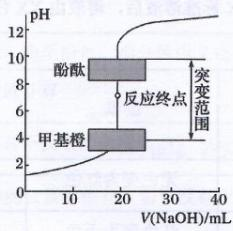
\includegraphics[max width=0.3\textwidth]{image/c5.jpg}
\end{center}

\subsection{小结}

\subsubsection{指示剂的选择原则}

①变色要明显、灵敏;

②指示剂的变色范围要尽可能在滴定过程中的 \(\mathrm{{pH}}\) 值突变范围内。

③指示剂用量不能太多, \(2 \sim 3\) 滴即可:

\subsubsection{指示剂的选择(由滴定曲线可知)}

①强酸强碱相互滴定, 可选用甲基橙或酚酞。

②若反应生成强酸弱碱盐, 溶液呈酸性, 则选用酸性变色范围的指示剂 (甲基橙);

若反应生成强碱弱酸盐, 溶液呈碱性, 则选用碱性变色范围的指示剂 (酚酞)

③石蕊试液因颜色变化不明显, 且变色范围过宽, 一般不作滴定指示剂。

④酸性 \({\mathrm{{KMnO}}}_{4}\) 溶液等本身呈现颜色的滴定试剂,不用另外选择指示剂

\subsubsection{终点判断}

 滴入最后半滴 XX 标准溶液后, 溶液由 XX 色突变 XX 色, 且半分钟内不褪色。

\begin{center}
	\adjustbox{max width=\textwidth}{
		\begin{tabular}{|c|c|c|}
			\hline
			指示剂 操作 & 酚酞 & 甲基橙 \\
			\hline
			强碱滴定强酸 & 无色变为红色 & 橙色变为黄色 \\
			\hline
			强酸滴定强碱 & 红色变为无色 & 黄色变为橙色 \\
			\hline
		\end{tabular}
	}
\end{center}

\subsection{误差分析}

以一元酸和一元碱的中的滴定为例

\[
{\mathrm{C}}_{\text{待 }}{\mathrm{V}}_{\text{待 }} = {\mathrm{C}}_{\text{标· }}{\mathrm{V}}_{\text{标 }}
\]

滴定过程中任何错误操作都有可能导致 \(\mathrm{C}\) 标、 \(\mathrm{V}\) 标、 \(\mathrm{V}\)待 的误差。但在实际操作中认为 \(\mathrm{C}\) 标是已

知的, \({\mathrm{V}}_{\text{待 }}\) 是固定的,对于 \({\mathrm{c}}_{\left( \mathrm{{NaOH}}\right) }  = \frac{{\mathrm{c}}_{\left( \mathrm{{HCl}}\right) }{\mathrm{V}}_{\left( \mathrm{{HCl}}\right) }}{{\mathrm{V}}_{(NaOH)} } \)


\[\mbox{读数比实际}\]

\subsection{误差分析}


\begin{center}
	\adjustbox{max width=\textwidth}{
		\begin{tabular}{|c|c|c|c|c|}
			\hline
			\phantom{X} & 产生误差的常见因素 & & 对 \(\mathrm{V}_{\mathrm{HCl}}\) 的影响 & 对 \(\mathbf{C}_{\mathrm{NaOH}}\) 的影响 \\
			\hline
			\multirow{4}{*}{滴定前操作} & 未用标准液润洗酸式滴定管 & [HCL]$\downarrow$& \(\uparrow\) & \(\uparrow\) \\
			\cline{2-5}
			& 未用待测液润洗碱式滴定管 &[NaOH]$\downarrow$& \(\downarrow\) & \(\downarrow\) \\
			\cline{2-5}
			& 用待测液润洗锥形瓶 &NaOH$\uparrow$& \(\uparrow\) & \(\uparrow\) \\
			\cline{2-5}
			& 洗涤后锥形瓶未干燥 &n(NaOH)不变& \(-\) & \(-\) \\
			\hline
			\multirow{2}{*}{滴定时读数不准} & 滴定前俯视酸式滴定管,滴定后平视 & & \(\uparrow\) & \(\uparrow\) \\
			\cline{2-5}
			& 滴定前仰视酸式滴定管,滴定后俯视&  & \(\uparrow\) & \(\uparrow\) \\
			\hline
			\multirow{2}{*}{取液时读数不准} & 取待测液时先俯视后仰视& & \(\downarrow\) & \(\downarrow\) \\
			\cline{2-5}
			& 取待测液时先仰视后俯视&  &\(\uparrow\) & \(\uparrow\) \\
			\hline
			\multirow{6}{*}{操作不当} & 滴定前酸式滴定管有气泡,滴定后气泡消失&  & \(\uparrow\) & \(\uparrow\) \\
			\cline{2-5}
			& 滴定前酸式滴定管无气泡,滴定后有气泡&  & \(\downarrow\) & \(\downarrow\) \\
			\cline{2-5}
			& 滴定结束,滴定管尖端挂一滴液体未滴下 & & \(\uparrow\) & \(\uparrow\) \\
			\cline{2-5}
			& 滴定过程中,振荡锥形瓶时,不小心将溶液溅出 & & \(\uparrow\) & \(\uparrow\) \\
			\cline{2-5}
			& 用甲基橙作指示剂,滴至橙色,半分钟内又还原成黄色,不处理就计算 & & \(\uparrow\) & \(\uparrow\) \\
			\cline{2-5}
			& 配制标准液的固体有不反应的杂质 & & \(\downarrow\) & \(\uparrow\) \\
			\hline
		\end{tabular}
}
\end{center}
%\end{comment}


\section{其他滴定}

\subsection{氧化还原滴定}

\subsubsection{酸性 \({\mathrm{{KMnO}}}_{4}\) 溶液滴定 \({\mathrm{H}}_{2}{\mathrm{C}}_{2}{\mathrm{O}}_{4}\) 溶液}

原理: \(2{\mathrm{{MnO}}}_{4}^{ - } + 6{\mathrm{H}}^{ + } + 5{\mathrm{H}}_{2}{\mathrm{C}}_{2}{\mathrm{O}}_{4} = {10}{\mathrm{{CO}}}_{2} \uparrow + 2{\mathrm{{Mn}}}^{2 + } + 8{\mathrm{H}}_{2}\mathrm{O}\) ;

指示剂及滴定终点: 酸性 \({\mathrm{{KMnO}}}_{4}\) 溶液本身呈紫红色,不用另外选择指示剂,当滴入最后半滴酸性 \({\mathrm{{KMnO}}}_{4}\) 溶液,溶液由无色变浅红色,且半分钟内不变色,说明达到滴定终点。

\subsubsection{ \({\mathrm{{Na}}}_{2}{\mathrm{\;S}}_{2}{\mathrm{O}}_{3}\) 溶液滴定碘液}

原理: \(2{\mathrm{\;S}}_{2}{\mathrm{O}}_{3}^{2 - } + {\mathrm{I}}_{2} = {\mathrm{S}}_{4}{\mathrm{O}}_{6}^{2 - } + 2{\mathrm{I}}^{ - }\) ;

指示剂及滴定终点: 用淀粉溶液+作指示剂,当滴入最后半滴 \({\mathrm{{Na}}}_{2}{\mathrm{\;S}}_{2}{\mathrm{O}}_{3}\) 溶液,溶液的蓝色褪去, 且半分钟内不恢复原色, 说明达到滴定终点。


\chapter{原电池}

\section{原电池}

\textit{将化学能转化为电能的装置, 本质为自发进行的氧化还原反应。}

\paragraph*{正极}

化合价$\downarrow$,得$e^{-}$$\Rightarrow$牺牲阳极的阴极保护法

\paragraph*{负极}

化合价$\uparrow$,失$e^{-}$,氧化反应

\subsection{原电池的构成条件}

1、活性不同的两极 
2、自发的氧化还原反应
3、闭合回路 
4、电解质

\section{盐桥}

\begin{center}
	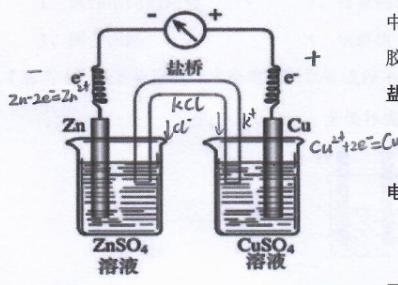
\includegraphics[max width=0.5\textwidth]{image/c14.jpg}
\end{center}

\subsection{盐桥构成}

盐桥里的物质一般是\dotuline{强电解质}而且不与两池中电解质反应, 常使用装有饱和 \(\mathrm{{KCl}}\) 琼脂溶胶的 \(\mathrm{U}\) 形管,离子可以在其中自由移动。

盐桥作用:

电极反应方程式: 

三大流向: 

\section{膜电池}

膜的引入简化了装置, 用离子交换膜分隔成两池, 仅允许特定的离子通过; 且膜能持续、长期使用。

\begin{center}
	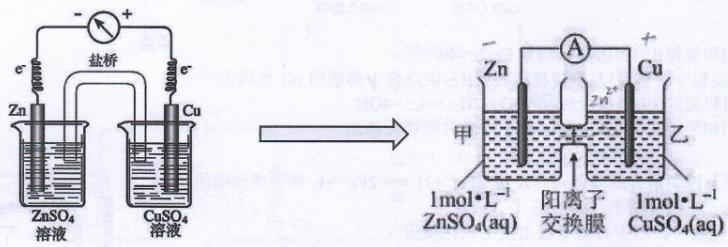
\includegraphics[max width=0.9\textwidth]{image/c16-1.jpg}
\end{center}

膜的分类:
 \textit{叫什么就只让什么离子过}

\ding{172}阳离子交换膜%圈1

\ding{173}阴离子交换膜

\ding{174}质子交换膜

只有$H^{+}$能过

\ding{175}双极膜

$H_{2}O\rightleftharpoons H^{+}+OH^{-}$一人去一边

\chapter{电解池}

%\section{电解池}

\begin{center}
	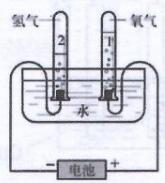
\includegraphics[max width=0.2\textwidth]{image/c19.jpg}
\end{center}

%请从电解水的能量变化和物质变换, 分析电解池的原理。

%\section*{电解池}

\textit{电解池: 把电能转变为化学能的装置。}

\paragraph{构成条件}~{}\\

1.电源

2.两个电极(只导电,可用惰性电极--石墨,铂Pt,金Au)

3.电解质(水/熔融)

4.闭合回路

\paragraph{两个电极}~{}\\

\subparagraph{阳极}
失去$e^{-}$化合$\uparrow$ 氧化反应
\subparagraph{阴极}
得$e^{-}$化合$\downarrow$ $\Rightarrow$\textbf{外加电源的阴极保护法}

\paragraph{流向}

\subparagraph*{电子}

阳$\rightarrow$阴

\subparagraph*{电流}

阴$\rightarrow$阳

\subparagraph*{$\star$离子}

异性相吸(阳离子$\rightarrow$阴极)

\section{电极反应方程式书写}

电极反应式: 电化学装置中表示原子或离子在电极上得失电子发生氧化或还原反应的式子

\subsection{电极方程式的书写步骤}

1.确定主要反应物和生成物

2.得(阴)/失(阳)  $e^{-}$数

3.环境离子(电荷守恒)

4.元素守恒配齐($H_{2}O$)

\section{溶液中的离子放电顺序}

\textbf{$\textreferencemark$由于各种离子得失电子的能力不同, 因此, 电解时离子放电难易也不同。}

\subsection{阴极上阳离子放电}

\paragraph*{氧化性}~{}\\

$Ag^{+} > Hg^{+} > Fe^{3+} > Cu^{2+} > H^{+}(\mbox{酸}) > Sn^{2+} > Fe^{2+} > Zn^{2+} > H^{+}(\mbox{水})$

$>Al^{3+} > Mg^{2+} > Na^{+} > Ca^{2+} > K^{+}$

\[\text{有}Cu^{2+} Ag^{+} \text{出}Cu,Ag\]
\[\text{无}Cu^{2+} Ag^{+} \text{出}H_{2},\text{放氢生碱}OH^{-}\]

\subsection{阳极上阴离子放电}

\paragraph*{还原性}~{}\\
	
	金属电极(除Pt,Au) > $S^{2-} > {SO_{3}}^{2-} > I^{-} > Br^{-} > Cl^{-} > OH^{}(\text{水/碱})\rightarrow O_{2}$
	
	
	>最高价含氧酸根${SO_{4}}^{2-},{CO_{3}}^{2-},{NO_{3}}^{-} > F^{-}$ 
	
	\[\text{有卤素出卤素}\]
	\[\text{无卤素出}O_{2},\text{放氧生酸}H^{+}\]
	
	
	
	% 定义 longtable 环境,表格有 4 列,每列内容居中对齐并用竖线分隔
	\begin{longtable}{|c|c|c|c|} 
		
		\hline % 表格顶部的横线
		
		% 表头部分
		\textbf{电解池情况} & \textbf{阳极产物} & \textbf{阴极产物} & \textbf{阳极: 阴极产物比例} \\ % 表头行,加粗列标题
		\hline % 表头行的下横线
		\endfirsthead % 结束表头部分的定义
		
		% 如果表格跨页,表头重复部分
		\hline % 表头行的上横线
		\textbf{电解池情况} & \textbf{阳极产物} & \textbf{阴极产物} & \textbf{阳极: 阴极产物比例} \\ % 表头行,加粗列标题
		\hline % 表头行的下横线
		\endhead % 结束表头重复部分的定义
		
		% 表格主体的底部横线
		\hline
		\endfoot % 结束表格主体的底部横线部分
		
		% 表格最后一页的底部横线
		\hline
		\endlastfoot % 结束表格最后一页的底部横线部分
		
		% 表格内容部分
		a.b 为铂电极, 硫酸钠溶液 & $O_{2}$ & $H_{2}$ & 1:2 \\ % 第一行数据
		\hline % 每行数据之后加横线
		a.b 为铂电极,硫酸铜溶液 & $O_{2}$ & Cu & 1:2 \\ % 第二行数据
		\hline
		a.b 为铂电极, 氯化铜溶液 & $Cl_{2}$ & Cu & 1:1\\ % 第三行数据
		\hline
		a, b 为铂电极,氯化钠溶液 & $Cl_{2}$ & $H_{2}$ & 1:1 \\ % 第四行数据
		\hline
		a, b 为铁电极, 氯化钠溶液 & $Fe^{2+}$ & $H_{2}$ & 1:1 \\ % 第五行数据
		\hline
	%	行6 & 数据16 & 数据17 & 数据18 \\ % 第六行数据
	%	\hline
		
	\end{longtable} % 结束 longtable 环境
	
	\subsection{阶段放电}
	
	$
	
	\left\{
	\begin{aligned}
		\text{足量XX溶液} \Rightarrow  	\text{无阶段(看溶液)} \\
		\text{少量/一定量XX溶液} \Rightarrow  	\text{顺序} \\
	\end{aligned}
	\right.
	$
	
	
	\section{电解池中膜的应用}
	
	
	\begin{center}
		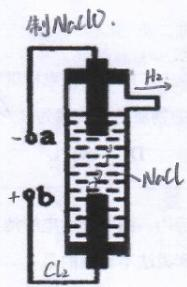
\includegraphics[max width=0.2\textwidth]{image/c26-1.jpg}
	\end{center}
	
	
	\begin{center}
	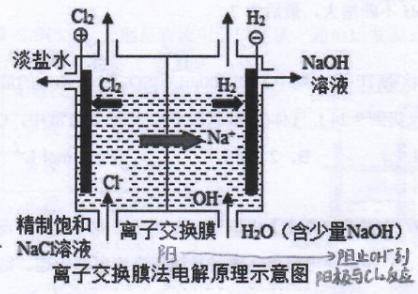
\includegraphics[max width=0.5\textwidth]{image/c26-2.jpg}
	\end{center}
	
	
	\subsection{离子交换膜}
	
	工业上氯碱工业利用离子交换膜来制备氯气和氢氧化钠;
	
	工业上利用离子交换膜进行\uwave{废水处理、海水淡化}等。
	
\section{二次电池}

二次电池又称可充电电池或蓄电池放电后可以充电使活性物质获得再生, 此类电池可重复使用。

\subsection{铅酸蓄电池}

稀硫酸

\({\mathrm{{PbO}}}_{2}\) (正极)

\(\mathrm{{Pb}}\) (负极)

放电时的电极方程式:

负极: \(\mathrm{{Pb}} + {\mathrm{{SO}}}_{4}{}^{2 - } - 2\mathrm{e} = {\mathrm{{PbSO}}}_{4}\)

正极: \({\mathrm{{PbO}}}_{2} + 4{\mathrm{H}}^{ + } + {\mathrm{{SO}}}_{4}{}^{2 - } + 2\mathrm{e} - = {\mathrm{{PbSO}}}_{4} + 2{\mathrm{H}}_{2}\mathrm{O}\)

总反应: \(\mathrm{{Pb}} + {\mathrm{{PbO}}}_{2} + 2{\mathrm{H}}_{2}{\mathrm{{SO}}}_{4} = 2{\mathrm{{PbSO}}}_{4} + 2{\mathrm{H}}_{2}\mathrm{O}\)

$\longleftarrow$电解池

\paragraph*{阳极}

$PbSO_{4} - 2e^{-} +2H_{2}O = PbO_{2} + 4H^{+} + {SO_{4}}^{2-}$
	\[\mbox{正接正(阳),负接负(阴)}\]
	\[\mbox{电极方程式完全相反},e^{-}\mbox{换边}\]
	
\subsection{锂离子电池}

 质量小、体积小、储存和输出能量大 (合金)
负极材料: 嵌锂石墨 正极材料: \({\mathrm{{LiCoO}}}_{2}\) (钴酸锂)

电解质溶液为 \({\mathrm{{LiPF}}}_{6}\) (六氟磷酸锂) 的碳酸酯溶液 (无水)

放电过程总反应为: \({\mathrm{{Lix}}}C\mathrm{y} + {\mathrm{{Li}}}_{1 - \mathrm{x}}{\mathrm{{CoO}}}_{2} \rightarrow {\mathrm{{LiCoO}}}_{2} + \mathrm{{Cy}}\)


\paragraph*{负极}

: \(\mathrm{{LixCy}} - \mathrm{{xe}} = {\mathrm{{xLi}}}^{ + } + \mathrm{{Cy}}\) 
\[{Li - {e}^{ - } = Li^{ + }\]

\paragraph*{正极}

 \({\mathrm{{Li}}}_{1 - \mathrm{x}}{\mathrm{{CoO}}}_{2} + {\mathrm{{xLi}}}^{ + } + {\mathrm{{xe}}}^{ - } = {\mathrm{{LiCoO}}}_{2}\) 
\[{\mathrm{{Li}}}^{ + } + {\mathrm{e}}^{ - } = \mathrm{{Li}}\]


\section{原电池与电解池的串联}

原电池电解池的串联: 利用原电池放电来作为电解池的电源。

	\[\mbox{先找原电池}\Rightarrow \mbox{电极活泼性/气体}\]
	\[\mbox{跨膜电子数}= \mbox{转移} e^{-}\]
	
	
	
\part{物质结构与性质}

\chapter{原子结构}
	

\section{原子构造原理发展历史}

\begin{center}
	\adjustbox{max width=\textwidth}{
		\begin{tabular}{|c|c|c|c|}
			\hline
			年份 & 国籍 & 科学家 & 贡献 \\
			\hline
			1814 年 & 德国 & 夫琅禾费 & 发明分光镜, 观察太阳光, 发现夫琅禾费线 \\
			\hline
			1859 年 & 德国 & 本生、基尔霍夫 & 证明夫琅禾费线是原子的吸收光谱, \\
			\hline
			1869 年 & 俄国 & 门捷列夫 & 发现元素周期表 \\
			\hline
			1913 年 & 丹麦 & 波尔 & 提出氢原子模型:电子在线性轨道绕核运行 \\
			\hline
			1918 年 & 丹麦 & 波尔 & 提出“能层”与“能级” \\
			\hline
			1920 年 & 丹麦 & 波尔 & 提出构造原理 \\
			\hline
			1926 年 & \multicolumn{3}{|c|}{量子力学} \\
			\hline
			1936 年 & 德国 & 马德隆 & 发表完整的构造原理 \\
			\hline
		\end{tabular}
	}
\end{center}

	
	\section{能层与能级}
	
	\paragraph*{能层}: 核外电子按照能量不同分成能层, \textit{能层越高, 电子离核越远, 电子的能量越高。}
	
	\begin{center}
		\adjustbox{max width=\textwidth}{
			\begin{tabular}{|c|c|c|c|c|c|c|c|}
				\hline
				能层 & 一 & 二 & 三 & 四 & 五 & 六 & 七 \\
				\hline
				符号 & \(\mathrm{K}\) & L & M & \(\mathrm{N}\) & O & P & Q \\
				\hline
				最多电子数 & 2 & 8 & 18 & 32 & 50 & 72 & 98 \\
				\hline
			\end{tabular}
		}
	\end{center}
	
	能量的高低顺序为: \(\mathrm{E}\left( \mathrm{K}\right) < \mathrm{E}\left( \mathrm{L}\right) < \mathrm{E}\left( \mathrm{M}\right) < \mathrm{E}\left( \mathrm{N}\right) < \mathrm{E}\left( \mathrm{O}\right) < \mathrm{E}\left( \mathrm{P}\right) < \mathrm{E}\left( \mathrm{Q}\right)\) 。
	
	能层=电子层
	
\paragraph*{能级}: 同一能层的电子, 还被分为不同能级, 每一能级所能容纳的电子数目也不同。能级的符号
	和所能容纳的最多电子数如下:
	
	\begin{center}
		\adjustbox{max width=\textwidth}{
			\begin{tabular}{|c|c|c|c|c|c|c|c|c|c|c|c|c|}
				\hline
				能层 & \(\mathbf{K}\) & \multicolumn{2}{|c|}{L} & \multicolumn{3}{|c|}{\(\mathbf{M}\)} & \multicolumn{4}{|c|}{\(\mathbf{N}\)} & \multicolumn{2}{|c|}{\(\mathbf{O}\)} \\
				\hline
				能 级 & 1s & 2s &2p & 3s &  3p & 3d &4s & 4p & 4d & 4f & 5s & 5p  \\
				\hline
				最多 电子数 & 2 & 2 &  6&  2&  6  & 10 &  2 & 6 & 10 & 14 &   2 & 6  \\
				\hline
			\end{tabular}
		}
	\end{center}
	
	\subparagraph*{s} $ 1 \times 2 $
	
	\subparagraph*{p} $ 3 \times 2 $
	
	\subparagraph*{d} $ 5 \times 2 $
	
	\subparagraph*{f} $ 7 \times 2 $
	
	
	\textit{能层数=具有的能级数}
	
\subsection{同能级比能层}
\[ns>(n-1)s>(n-2)s>(n-3)s\]

\section{构造原理和电子排布式}

\subsection{构造原理}
	
	以光谱学事实为基础, 从氢开始, 随核电荷数递增, 新增电子填入能级的顺序称为构造原理。
	
	\begin{center}
		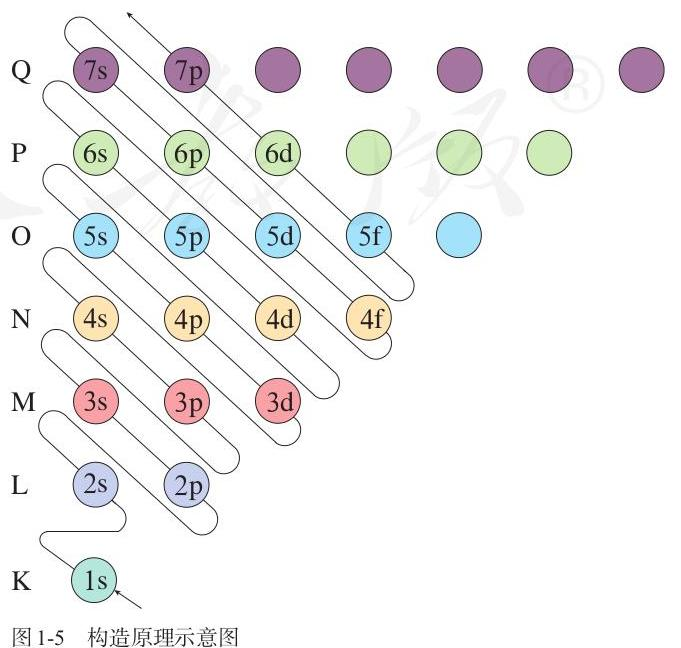
\includegraphics[max width=0.5\textwidth]{image/c43-2.jpg}
	\end{center}
	
	\subsection{能级交错}
	\paragraph*{原理:} 电子总是占据能量较低的能级。
	
	\paragraph*{影响因子 1:} 占据能量较 高能级使整体能量升高。
	
	\paragraph*{影响因子 2: }同一能级电子排斥使整体能量升高。
	
	\textit{当相邻两个能级能量相差不大, 电子排斥能大于两个能级之间能量差距, 电子填充能量较高能级, 出现能级交错。}
		\begin{center}
		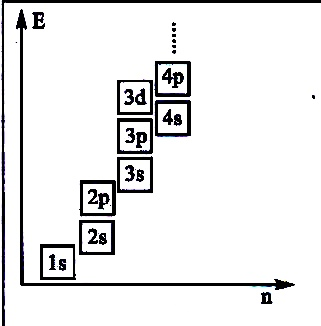
\includegraphics[max width=0.5\textwidth]{image/c43-1.jpg}
	\end{center}
	
	
	按照构造原理, 电子填满一个能级, 开始填入下一个能级, 由此构建了元素周期表中各元素的基态原子的电子排布。
	
		\begin{center}
		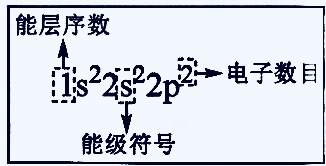
\includegraphics[max width=0.3\textwidth]{image/c44.jpg}
	\end{center}
	
	
	4s<3d能量
	
			$
	
	\left\{
	\begin{aligned}
		\text{书写:先3d再4s}  \\
		\text{得失}e^{-}   \text{先4s再3d}\\
	\end{aligned}
	\right.
	$
	
	\subsection{屏蔽效应}
	
	由于其他电子对某一电子的排斥作用而抵消了一部分核电荷对该电子的吸引力. 从而引起有效核电荷的降低, 削弱了核电荷对该电子的吸引, 这种作用称为屏蔽作用或屏蔽效应。
	
	\paragraph*{价电子层}在化学反应中可能发生电子变动的能级称为价电子层 (简称价层)。
	\paragraph*{简化电子排布式} [前一周期稀有气体符号]价层电子排布。 (3d不含在Ar里面)
	
	\section{基态与激发态原子光谱}
	
	\paragraph*{基态原子:} 处于最低能量状态的原子叫做基态原子。
	
	\paragraph*{激发态原子:} 基态原子吸收能量, 它的\uwave{电子会跃迁到较高能级}(\uline{只能跳到相邻层级}), 变为激发态原子。
	
	电子从较高能量的激发态跃迁到较低能量的激发态乃至基态时, 将释放能量 (主要以光的形式)。
	
	\subsection{原子光谱}
	
	不同元素原子的电子发生跃迁时会吸收或释放不同的光, 可以用光谱仪摄取各种元素原子的吸收光谱或发射光谱, 总称原子光谱。
	\subsubsection{原子吸收光谱}
	
	电子由低能级向高能级发生跃迁, 会吸收一定波长的光线, 因此会在全光谱上留下相应的暗线, 称为原子吸收光谱。
	
	基 \(  \rightarrow   \) 激
	
	\subsubsection{原子发射光谱}
	
	电子由高能级向低能级发生跃迁, 会释放一定波长的光线, 称为原子发射光谱。
	
	在现代化学中, 常利用原子光谱上的特征谱线来鉴定元素, 称为光谱分析。
	
	激$\rightarrow$基  焰色试验
	\subsubsection*{日常应用}
	
	 焰火、霓虹灯光、激光、萤光、LED 灯光等。
	 
\chapter{电子云与原子轨道}
	 
	 概率密度: 用 \(\mathrm{P}\) 表示电子在某处出现的概率, \(\mathrm{V}\) 表示该处的体积,则 \(\mathrm{P}/\mathrm{V}\) 称为概率密度,用 \(\rho\) 表示。
	 
	 	\begin{center}
	 	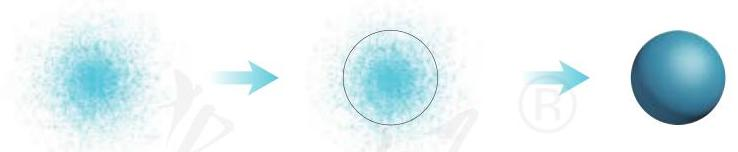
\includegraphics[max width=0.5\textwidth]{image/c51-1.jpg}
	 \end{center}
	 \section{电子云 }
	 
	 由于核外电子的\uwave{概率密度分布}看起来像一片云雾, 因而被形象地称作电子云。
	 
	 \section{电子云轮廓图}
	 
	 把电子在原子核外空间出现概率 \(\mathrm{P} = {90}\%\) 的空间圈出来,得到电子云轮廓图。 
	 
	 \section{电子云轮廓图形状}
	 
	\subsection{s电子云轮廓图}
	
	 \uwave{球形},且能层序号越大,半径越大。
	 
	 	\begin{center}
	 	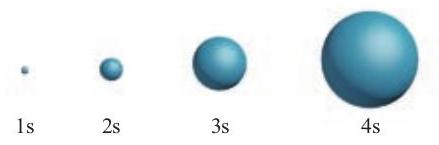
\includegraphics[max width=0.5\textwidth]{image/c51-2.jpg}
	 \end{center}
	 
	 \subsection{p 电子云轮廓图} 
	 
	 \uwave{哑铃形},且有三个互相垂直的电子云
	 
	 $P_{x},P_{y},P_{z}$能量相同
	 
	 	\begin{center}
	 	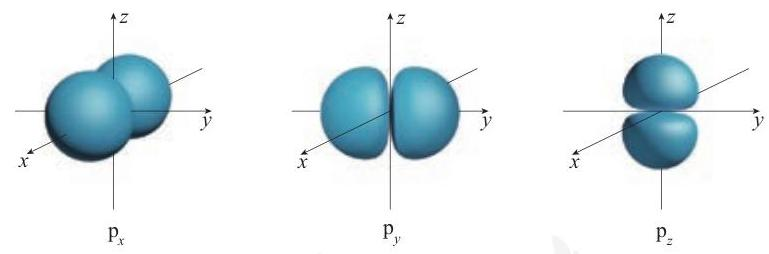
\includegraphics[max width=0.5\textwidth]{image/c51-3.jpg}
	 \end{center}
	 
	 \section{钻穿效应} 
	 
	 在原子核附近出现的概率较大的电子, 可更多地避免其余电子的排斥, 受到核的较强的吸引而更靠近核, 这种进入原子内部空间的作用叫做钻穿效应, 钻穿效应可以使能级降低。
	 
	 \section{原子轨道}
	 
	 量子力学把电子在原子核外的一个空间运动状态称为一个原子轨道。
	 
	 每一个轨道最多容纳两个电子, \(\mathrm{s}\) 能级包含 1 个轨道, \(\mathrm{p}\) 能级包含 3 个轨道, \(\mathrm{d}\) 能级包含 5 个轨道, \(f\) 能级包含 7 个轨道
	 
	 \begin{center}
	 	\adjustbox{max width=\textwidth}{
	 		\begin{tabular}{|c|c|c|c|c|}
	 			\hline
	 			能级 & ns & np & nd & nf \\
	 			\hline
	 			轨道数目 & 1 & 3 & 5 & 7 \\
	 			\hline
	 			最多容纳电子数 & 2 & 6 & 10 & 14 \\
	 			\hline
	 		\end{tabular}
	 	}
	 \end{center}
	 
	 \chapter{泡利原理、洪特原理、能量最低原理}
	 
	 轨道表示式: 用方框 (也可用圆圈) 表示原子轨道, 能量相同的原子轨道称为简并轨道。
	 
	 自旋: 电子除空间运动状态外, 还有一种状态叫自旋。电子自旋在空间有顺时针和逆时针两种取向,简称自旋相反,常用上下箭头 \(\left( { \uparrow \text{和} \downarrow }\right)\) 表示自旋相反的电子。
	 
	 \section{ 洪特规则}
	 \textit{ 基态原子中, 填入简并轨道的电子总是\uwave{先单独分占, 且自旋平行}, 称为洪特规则。}
	  
	  	 \begin{center}
	  	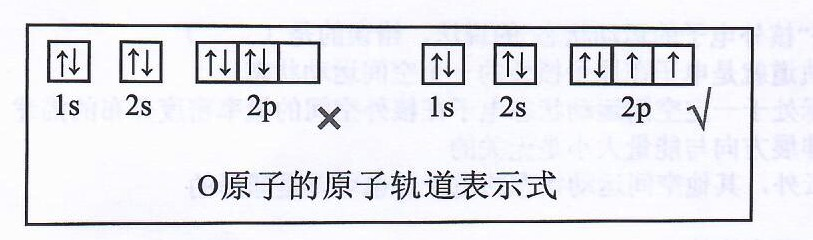
\includegraphics[max width=0.6\textwidth]{image/c54-1.jpg}
	  \end{center}
	  
	 \section{泡利原理}
	 
	 \textit{\uwave{在一个原子轨道里, 最多只能容纳两个电子, 他们的自旋相反}, 这个原理被称为泡利原理。}
	
	 	 \begin{center}
	 	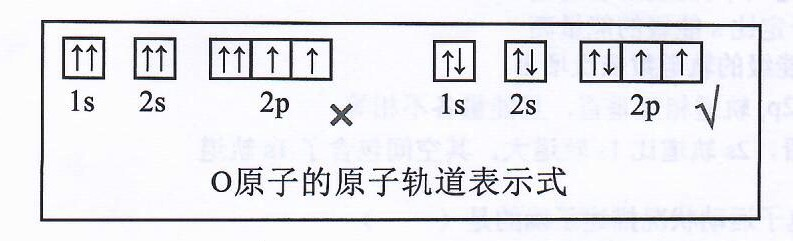
\includegraphics[max width=0.6\textwidth]{image/c54-2.jpg}
	 \end{center}

	 
	 \section{能量最低原理}
	 
	  在构建基态原子时, 电子将尽可能占据能量最低的原子轨道, 使整个原子的能量最低,这就是能量最低原理。 
	  
	  半满/全满 能量最低
	 
	 \begin{center}
	 	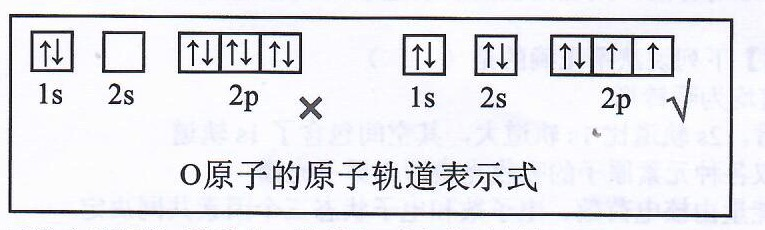
\includegraphics[max width=0.6\textwidth]{image/c54-3.jpg}
	 \end{center}
	 
	 \textit{基态原子的核外电子排布遵循泡利原理、洪特规则和能量最低原理。}
	 
	 
	 
\end{document}